% =============================================================================
% gp-posterior.tex — Gaussian process posterior mean with uncertainty band
%
% Shows: posterior mean curve, 95%-band that narrows near observed points,
% and the three observations themselves. Hand-drawn axes (no pgfplots
% dependency — matches the plain-TikZ convention used by regression-scatter.tex).
% Compiles standalone via: xelatex gp-posterior.tex
% =============================================================================

\documentclass[border=4pt]{standalone}
\usepackage{tikz}
\usetikzlibrary{arrows.meta}

\definecolor{mean}{HTML}{012169}
\definecolor{band}{HTML}{E8EDF5}
\definecolor{obs}{HTML}{B23A48}
\definecolor{axis}{HTML}{1A1A1A}

% -----------------------------------------------------------------------------
% Diagram: GP posterior over x in [0, 10], y in [-0.3, 6].
% Mean values at x = 0..10 (integer grid): 2.0, 2.8, 3.0, 3.6, 4.0, 4.5, 3.8,
%   3.0, 2.5, 2.0, 1.6 — the wiggle is illustrative, not fit to real data.
% Half-band width at the same grid: 1.3, 1.0, 0.25, 0.7, 0.95, 0.25, 0.75,
%   1.0, 0.25, 0.85, 1.3 — narrow exactly at the three observations (x = 2,
%   5, 8), wide away from them, the qualitative GP signature.
% -----------------------------------------------------------------------------

\begin{document}
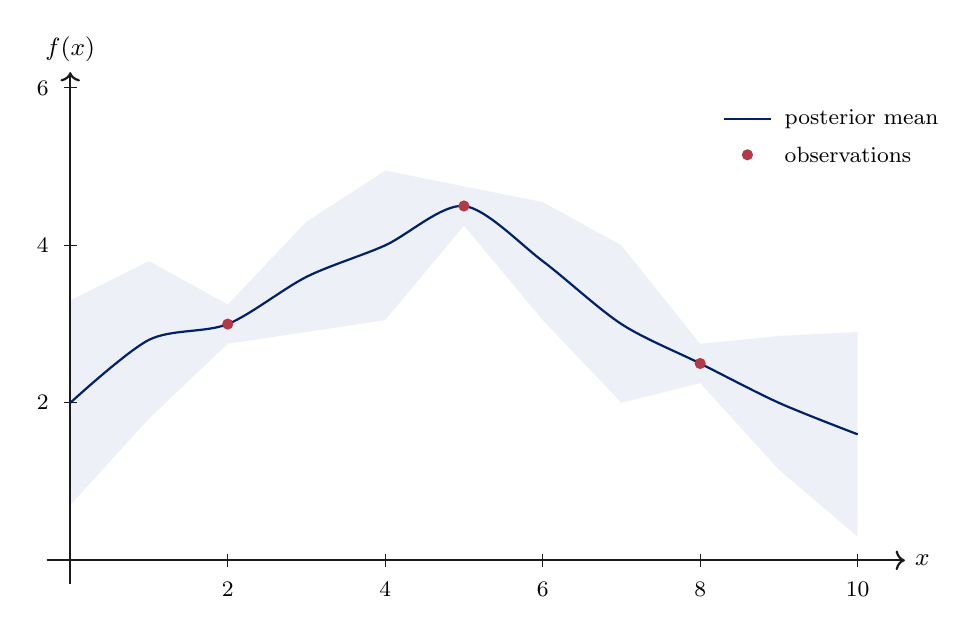
\begin{tikzpicture}
  % Uncertainty band (upper edge left-to-right, then lower edge right-to-left)
  \fill[band, opacity=0.8]
    (0,3.3) -- (1,3.8) -- (2,3.25) -- (3,4.3) -- (4,4.95) -- (5,4.75)
    -- (6,4.55) -- (7,4.0) -- (8,2.75) -- (9,2.85) -- (10,2.9)
    -- (10,0.3) -- (9,1.15) -- (8,2.25) -- (7,2.0) -- (6,3.05)
    -- (5,4.25) -- (4,3.05) -- (3,2.9) -- (2,2.75) -- (1,1.8) -- (0,0.7)
    -- cycle;

  % Axes
  \draw[->, thick, draw=axis] (-0.3, 0) -- (10.6, 0) node[right] {\small $x$};
  \draw[->, thick, draw=axis] (0, -0.3) -- (0, 6.2) node[above] {\small $f(x)$};

  % Tick marks
  \foreach \x in {2, 4, 6, 8, 10} {
    \draw[draw=axis] (\x, -0.08) -- (\x, 0.08);
    \node[below, font=\footnotesize] at (\x, -0.15) {\x};
  }
  \foreach \y in {2, 4, 6} {
    \draw[draw=axis] (-0.08, \y) -- (0.08, \y);
    \node[left, font=\footnotesize] at (-0.15, \y) {\y};
  }

  % Posterior mean
  \draw[thick, draw=mean] plot[smooth] coordinates {
    (0,2.0) (1,2.8) (2,3.0) (3,3.6) (4,4.0) (5,4.5)
    (6,3.8) (7,3.0) (8,2.5) (9,2.0) (10,1.6)
  };

  % Observations — band pinches to near-zero width here
  \foreach \x/\y in {2/3.0, 5/4.5, 8/2.5} {
    \filldraw[obs] (\x, \y) circle (1.8pt);
  }

  % Legend — placed in the empty upper-right corner, clear of the band and curve
  \draw[thick, draw=mean] (8.3, 5.6) -- (8.9, 5.6);
  \node[right, font=\footnotesize] at (8.95, 5.6) {posterior mean};
  \filldraw[obs] (8.6, 5.15) circle (1.8pt);
  \node[right, font=\footnotesize] at (8.95, 5.15) {observations};
\end{tikzpicture}
\end{document}
